
\chapter{STABILITY AND RECONSTRUCTIONS OF PT/PD BIMETALLIC NANOCUBES EXPOSED TO CARBON MONOXIDE}

\section{Introduction}

While metal surfaces are used in various industrial processes, because of their
poor surface area to volume ratio, many methods make use of roughened surfaces
or more preferrably nanoparticles dispersed on a cheaper unreactive
surface.\cite{Munnik:2015qf, Graham:2007ng} The size distribution of the
nanoparticles can vary but tends to be on the order of tens to hundredes of
nanometers in size.\citep{Zhang:2011ne, Liu:2013hf} Additionally, the
morphology of these nanoparticles spans from simple cubes, to octahedra,
pyramids, and numerous other morphologies.\citep{Ahmadi:2015os, Wang:2015qb,
Wang:2016dg} As seen in previous work\citep{Tao:2010aa, Michalka:2013aa,
Michalka:2015aa, Kim:2016cr}, even fairly stable surfaces can undergo large
scale reconstructions under experimental conditions. This appendix provides
information on the initial setup of bimetallic Pt/Pd nanocubes and the
preliminary results obtained before the project was shelved. 

\section{Methodology}
\subsection{Interaction Parameters}
The interaction potentials provided in Michalka {\em et
al.}\citep{Michalka:2015aa} are used here unchanged. 

\subsection{System Details}
Nanocubes with edge lengths of 6, 7, and 8 nm were constructed from an ideal
\ce{Pd} FCC lattice with a lattice constant of 3.89 \AA~  and cut so as to
expose the (100), (010), and (001) facets. For each of these three sizes, the
outermost 1, 2, or 3 layers were further replaced with Pt to create nine total
systems whose compositions are depicted in table \ref{tab:systems}. Work by Cao
{\it et al.}\citep{Cao:2010gf} on the self-distillation of bimetallic
nanostructures showed that when the outer shell of nanoparticles was composed
of the metal with a higher melting temperature, it imposed stability on the
confined inner metal. For this reason, Pt was chosen to compose the outer
layers while keeping the core of the nanoparticle Pd. Additionally, the
slightly more favorable Pd-CO interaction may provide a driving force for
reconstructions that will be dependent on the thickness of the Pt since Pd will
want to migrate through the Pt to the surface.

\begin{table}
  \caption{PT/PD NANOCUBE SIZES AND COMPOSITION}
  \centering
  \begin{threeparttable}
  \begin{tabular}{ c ccc }
  \hline
  \hline
  \textbf{System} & \textbf{Pd} & \textbf{Pt} &  \textbf{(Pt/total)} \\
  \hline
  6nm-1L & 10976 & 2524  & 0.187 \\
  6nm-2L & 8788  & 4712  & 0.349 \\
  6nm-3L & 6912  & 6588  & 0.488 \\
  7nm-1L & 19652 & 3676  & 0.157 \\
  7nm-2L & 16384 & 6944  & 0.298 \\
  7nm-3L & 13500 & 9828  & 0.421 \\
  8nm-1L & 27436 & 4564  & 0.143 \\
  8nm-2L & 23328 & 8672  & 0.271 \\
  8nm-3L & 19652 & 12348 & 0.386 \\
  \hline
  \hline
  \end{tabular}
  \end{threeparttable}
\label{tab:systems}
\end{table}

Systems were constructed in a non-periodic box and then initially equilibrated
at 5~K to allow the slight strain of replacing Pd atoms with Pt in the outer
layers to dissipate. Warming over approximately 3~ns was performed to bring all
systems up to a simulation temperature of 1000~K at which point an amount of
Carbon Monoxide equivalent to a 0.5 ML coverage was introduced into the system.
After another brief period of equilibration during which a significant amount
of the CO adsorbed to the surface, the systems were then run in the
microcanonical (NVE) ensemble for an additional 3~ns of data production.

Figures \ref{fig:6nm}, \ref{fig:7nm}, and \ref{fig:8nm} highlight the nanocube
systems after the initial strain relaxation and then after the systems have
been warmed. The instability of the smaller systems as highlighted in Figures
\ref{fig:6nm}, \ref{fig:7nm}.a, and \ref{fig:8nm}.a is one the reasons this project was paused.
Specifically, the 6nm systems underwent extreme distortions
from the nanocube morphology during the warming procedure and even at 750~K as
displayed in the image, the original (100) surface has almost entirely been
replaced with the more stable (111) surface. The larger mass of the 7 and 8nm
systems allowed for a greater amount of stability; however, the 1L systems for
both sizes still experienced an extremely large amount of restructuring.

\begin{landscape}
\begin{figure}[p!]
\centering
  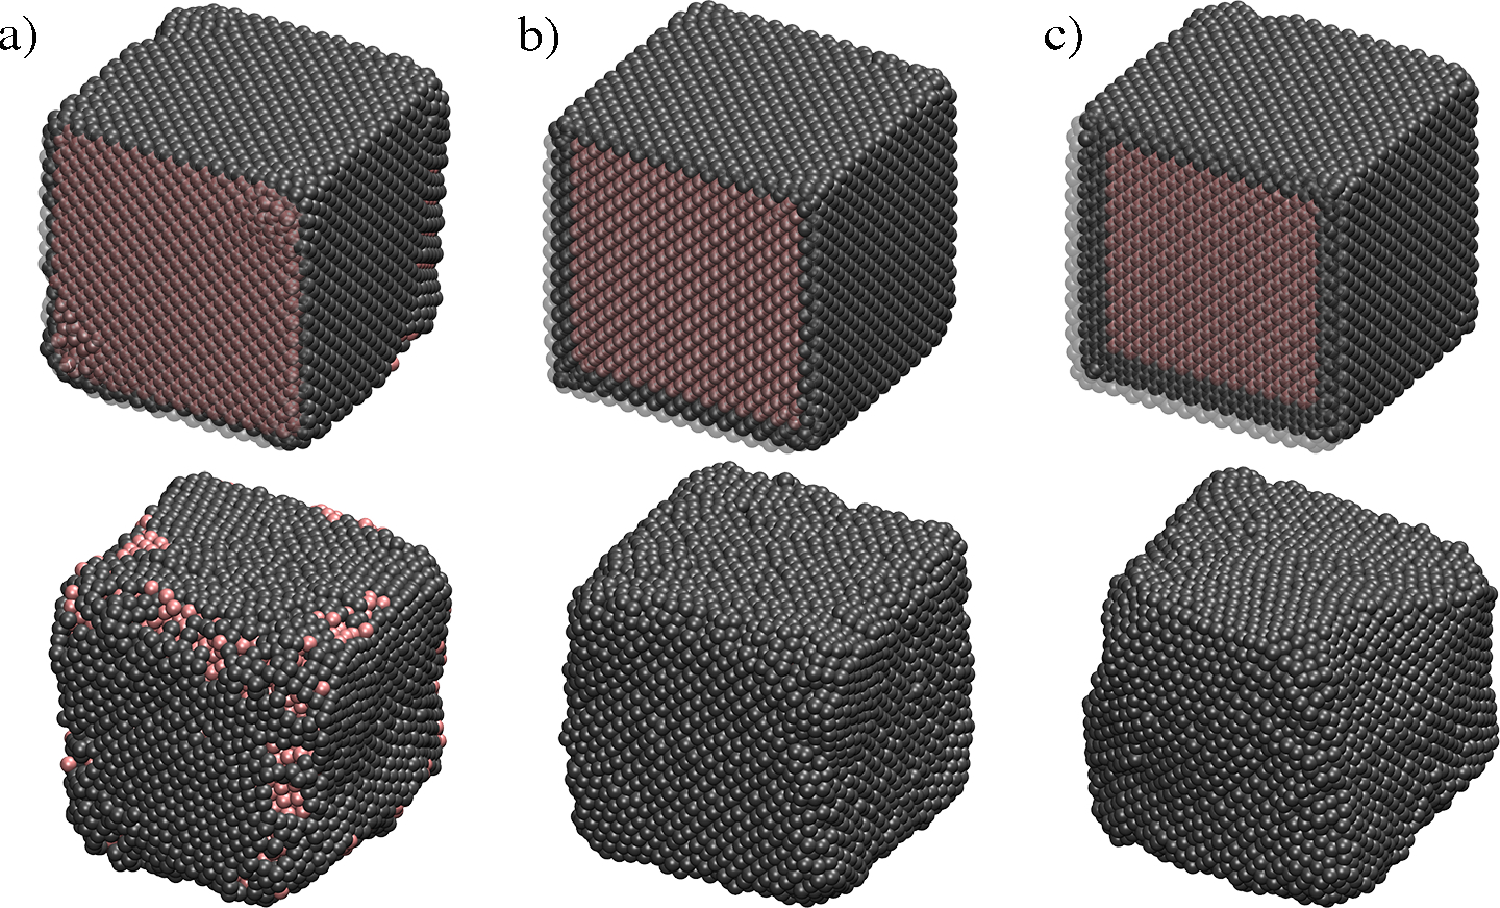
\includegraphics[width=0.8\linewidth]{../figures/appB/6nm.pdf}
  \caption{The top row images display the 6 nm nanocubes after warming the
systems to 300~K. \ce{Pt} atoms are gray while \ce{Pd} atoms are pink and the
there is a slight transparency of the front \ce{Pt} face to show the inner
\ce{Pd} atoms. The bottom row depict the same systems after warming to 750~K.
(a) corresponds to the one-layer (1L) system while (b) and (c) correspond to
the 2L and 3L systems respectively. }
  \label{fig:6nm}
\end{figure}
\end{landscape}

\begin{landscape}
\begin{figure}[p!]
\centering
  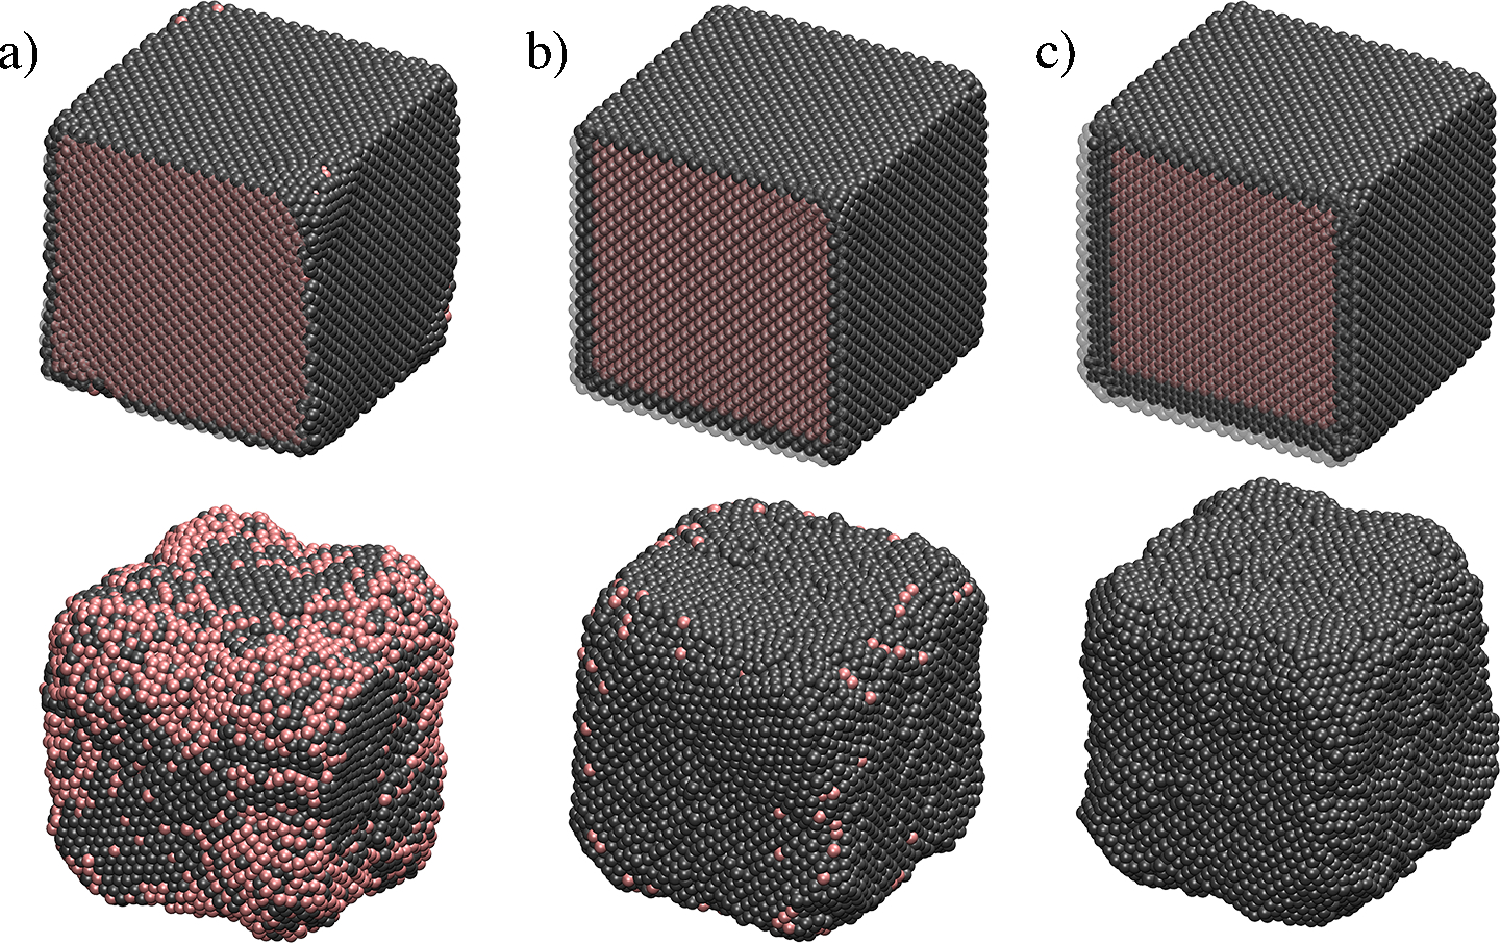
\includegraphics[width=0.8\linewidth]{../figures/appB/7nm.pdf}
  \caption{The top row images display the 7 nm nanocubes after warming the
systems to 300~K.  The bottom row depict the same systems after warming to
1000~K.  (a) corresponds to the one-layer (1L) system while (b) and (c)
correspond to the 2L and 3L systems respectively. The 7nm-1L system is somewhat
unstable and shows significant deviations away from the original (100) facets.}
  \label{fig:7nm}
\end{figure}
\end{landscape}

\begin{landscape}
\begin{figure}[p!]
\centering
  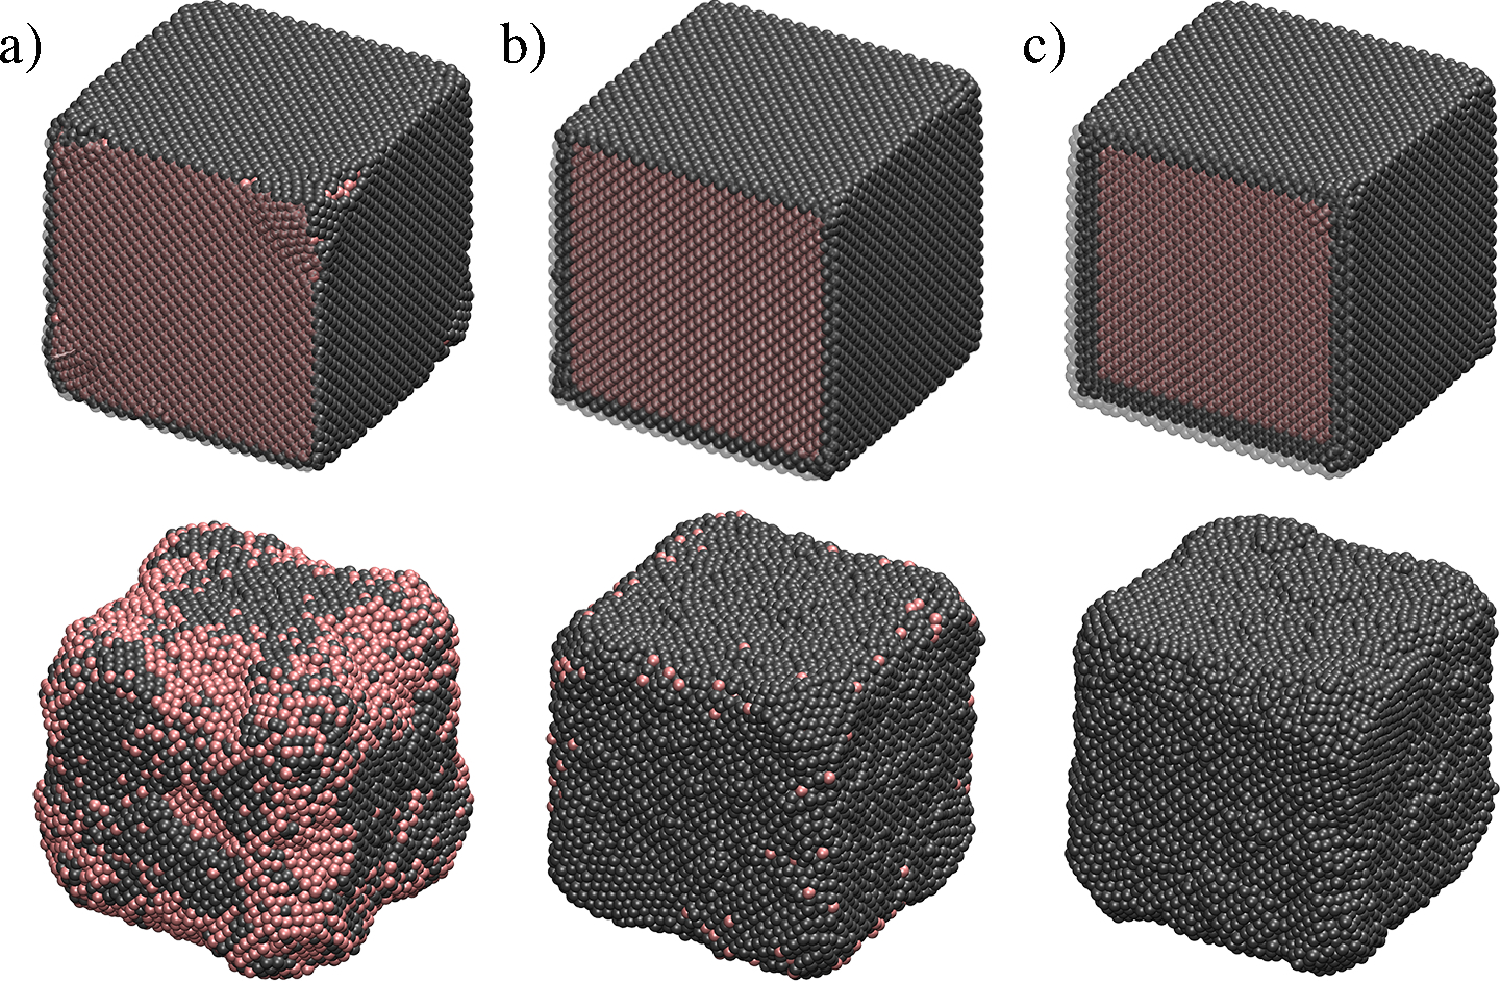
\includegraphics[width=0.8\linewidth]{../figures/appB/8nm.pdf}
  \caption{The top row images display the 8 nm nanocubes after warming the
systems to 300~K.  The bottom row depict the same systems after warming to
1000~K.  (a) corresponds to the one-layer (1L) system while (b) and (c)
correspond to the 2L and 3L systems respectively. Similar to the 7nm-1L system,
the 8nm-1L nanocube undergoes signficant restructuring to maximize the
formation of (111) domains on the surface. }
  \label{fig:8nm}
\end{figure}
\end{landscape}



\section{Results \& Discussion}
Another one of the challenges that ultimately led to this project being shelved
is the size of the systems and the cocommitant increase in simulation time
needed to capture the hypothesized restructuring processes. Nevertheless,
preliminary results were gathered and are discussed below.

\subsection{CO-Induced Reconstruction}
As seen in previous work\citep{Michalka:2013aa}, the presence of CO was again
seen to play a role in the observed restructuring. However, unlike what was
observed on the \ce{Pt} (557) surface, where \ce{CO} was
required for any large-scale reconstruction to occur, for these systems a
significant portion of the reconstruction could be directly attributed to lower
stability of the (100) facets when compared to (111) facets. As highlighted in
Figure \ref{fig:6nm}, these systems underwent the extreme amount of
reconstruction despite no CO being present. 

However, specifically examining Figure \ref{fig:8nmCO}.b shows that the
preferred Pd-CO binding does lead to a diffusion of the inner Pd to the surface
of the nanocube. The areas with the most reconstruction appear to be the edges
and corners of the cubes which is well understood as the atoms at those sites
tend to be undercoordinated and thus are easier to diffuse to a lower energy
configuration. 

Surface energy arguments could also be made to explain some of the
restructuring since in the EAM forcefield that is being used to describe the
metal-metal interactions, a Pt-Pd bond is more favorable than a Pd-Pd bond.
Thus, given time and energy to overcome kinetic barriers, all of the Pt on the
surface would like to be subsumed underneath the Pd. However, a Pt-Pt is
stronger still and there is a possibility that a sintering mechanism might
occur to maximize the number of ``bulk'' Pt.


\begin{landscape}
\begin{figure}[p!]
\centering
  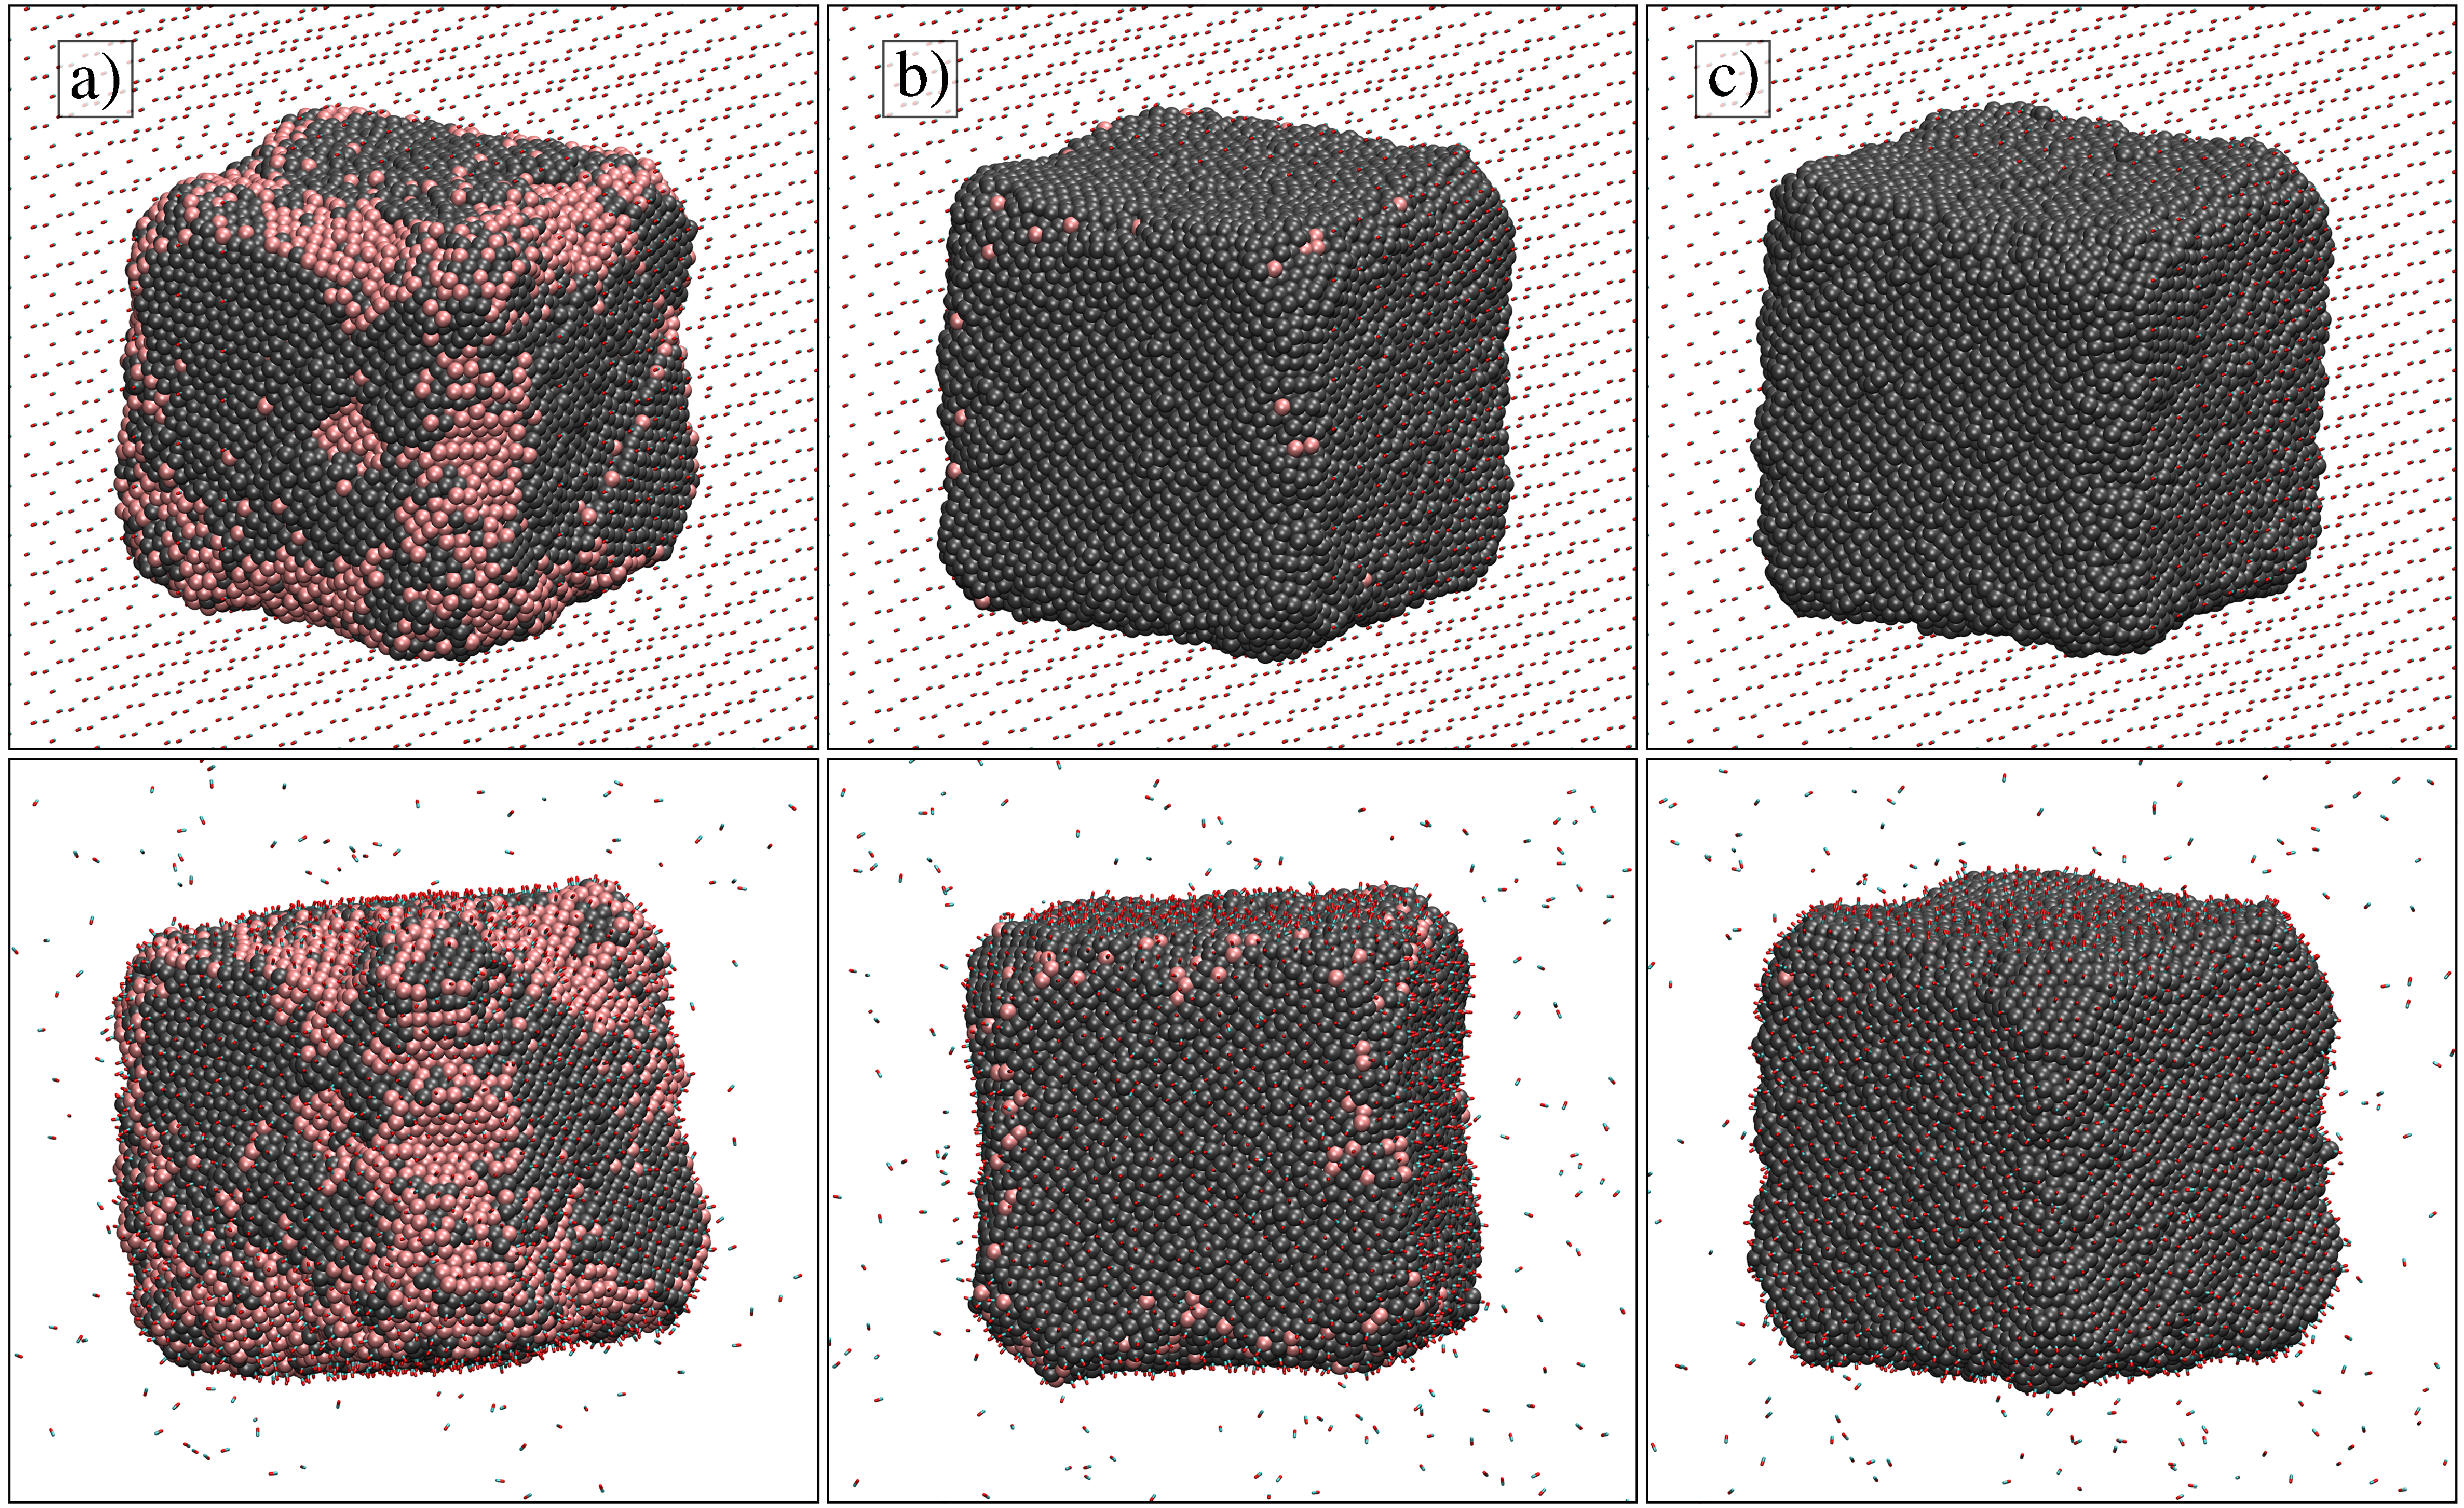
\includegraphics[width=0.8\linewidth]{../figures/appB/8nm_CO.pdf}
  \caption{The top row images depict the 8nm nanocubes surrounded by the
equivalent of a 0.5 ML of CO. The bottom row shows the same systems after 3 ns.
The small amount of rotation is due to an improperly sampled velocity
distribution of the CO which upon adsorption and collision with the nanocube
imparted a slight rotation.}
  \label{fig:8nmCO}
\end{figure}
\end{landscape}



\section{Summary}
The observed restructuring while informative, was primarily determined to be an
artifact of the small system sizes that were chosen for this investigation.
Future simulations examining larger systems (>10 nm) may solve the buckling
observed in a number of these systems. Additionally, an exploration into
octahedral-type nanoparticles with their preferred (111) facets may also help
solve the stability issues and provide another direction to explore.
